\begin{center}
\section{METODOLOGÍA, ACTIVIDADES Y CRONOGRAMA}
\end{center}

\subsection{METODOLOGÍA}
La metodología que se utilizará como referencia en el desarrollo del trabajo de grado en modalidad práctica profesional es la metodología del PMI. Este tipo de metodología proporciona un desarrollo del proyecto de manera gradual en la ejecución de los objetivos propuestos a través de procesos que se mencionan a continuación: Proceso de iniciación, Proceso de planificación, Proceso de ejecución, Proceso de supervisión y control, Proceso de cierre del proyecto.

\subsection{FASES Y ACTIVIDADES}
\begin{longtable}[htbp]{|p{4.055em}|p{11.22em}|p{20em}|}
  \caption{Fases y Actividades} \\
  \hline
  \multicolumn{1}{|c|}{\textbf{FASE}} & \textbf{NOMBRE} & \textbf{ACTIVIDADES} \bigstrut\\
  \hline
  \endfirsthead
  \multicolumn{3}{c}%
  {\tablename\ \thetable\ -- \textit{Fases y Actividades}} \\
  \hline
  \multicolumn{1}{|c|}{\textbf{FASE}} & \textbf{NOMBRE} & \textbf{ACTIVIDADES} \bigstrut\\
  \hline
  \endhead
  \hline
  \multicolumn{3}{r}{\textit{Continúa en la siguiente página}} \\
  \endfoot
  \hline
  \endlastfoot
  \multirow{4}{*}{\centering\textbf{I}} & Proceso de iniciación & 
  1. Recopilar información sobre prácticas de seguridad en la empresa WIZIT MIND BLOWING SOLUTIONS S.A.S, y sobre la norma ISO 27001: Realizar entrevistas o reuniones con representantes de la empresa para conocer las prácticas de seguridad actuales, los procedimientos implementados y las políticas establecidas. \newline{}
  2. Identificar los sistemas y aplicaciones desarrollados en Node.js: Obtener un inventario de las plataformas y aplicaciones desarrolladas en Node.js por la empresa, así como su importancia y criticidad. \newline{}
  3. Analizar las vulnerabilidades comunes en aplicaciones web con Node.js: Realizar una revisión de la literatura y recopilar información sobre las vulnerabilidades más frecuentes que afectan a las aplicaciones web desarrolladas en Node.js. \newline{}
  4. Definir el alcance y los objetivos específicos del proyecto: Asegurarse de que los objetivos establecidos anteriormente sean claros y alineados con las necesidades de la empresa WIZIT MIND BLOWING SOLUTIONS S.A.S. \bigstrut\\
  \hline
  \multirow{3}{*}{\centering\textbf{II}} & Proceso de Planificación & 
  5. Establecer el alcance del proceso, indicando qué aplicaciones y plataformas de la empresa estarán cubiertas por el esquema de seguridad en capas.\newline{}
  6. Identificar las capas de seguridad y las medidas correspondientes.\newline{}
  7. Establecer criterios de selección de tecnologías y herramientas disponibles para el desarrollo con Node.js. \bigstrut\\
  \hline
  \multirow{3}{*}{\centering\textbf{III}} & Proceso de Ejecución & 
  8. Implementar las capas de seguridad seleccionadas, con las medidas de seguridad correspondientes en cada capa.\newline{}
  9. Implementar las herramientas y tecnologías de seguridad elegidas durante la fase de planificación.\newline{}
  10. Elaborar documentación detallada que describa las medidas de seguridad implementadas en cada capa, para su correcta aplicación en la empresa WIZIT MIND BLOWING SOLUTIONS S.A.S. \bigstrut\\
  \hline
  \multirow{2}{*}{\centering\textbf{IV}} & Proceso de Supervisión & 
  11. Evaluar el estado de seguridad de las aplicaciones y verificar la efectividad de las medidas implementadas.\newline{}
  12. Documentar los hallazgos, identificar áreas de mejora y proponer acciones correctivas o preventivas. \bigstrut\\
  \hline
  \multirow{3}{*}{\centering\textbf{V}} & Proceso de Cierre del Proyecto & 
  13. Entrega de documentos (Documento final y archivos del modelo replicable).\newline{}
  14. Entrega del modelo de seguridad en capas a la empresa WIZIT MIND BLOWING SOLUTIONS S.A.S.\newline{}
  15. Preparación y realización de la sustentación. \bigstrut\\
  \hline
\end{longtable}


\begin{landscape}
  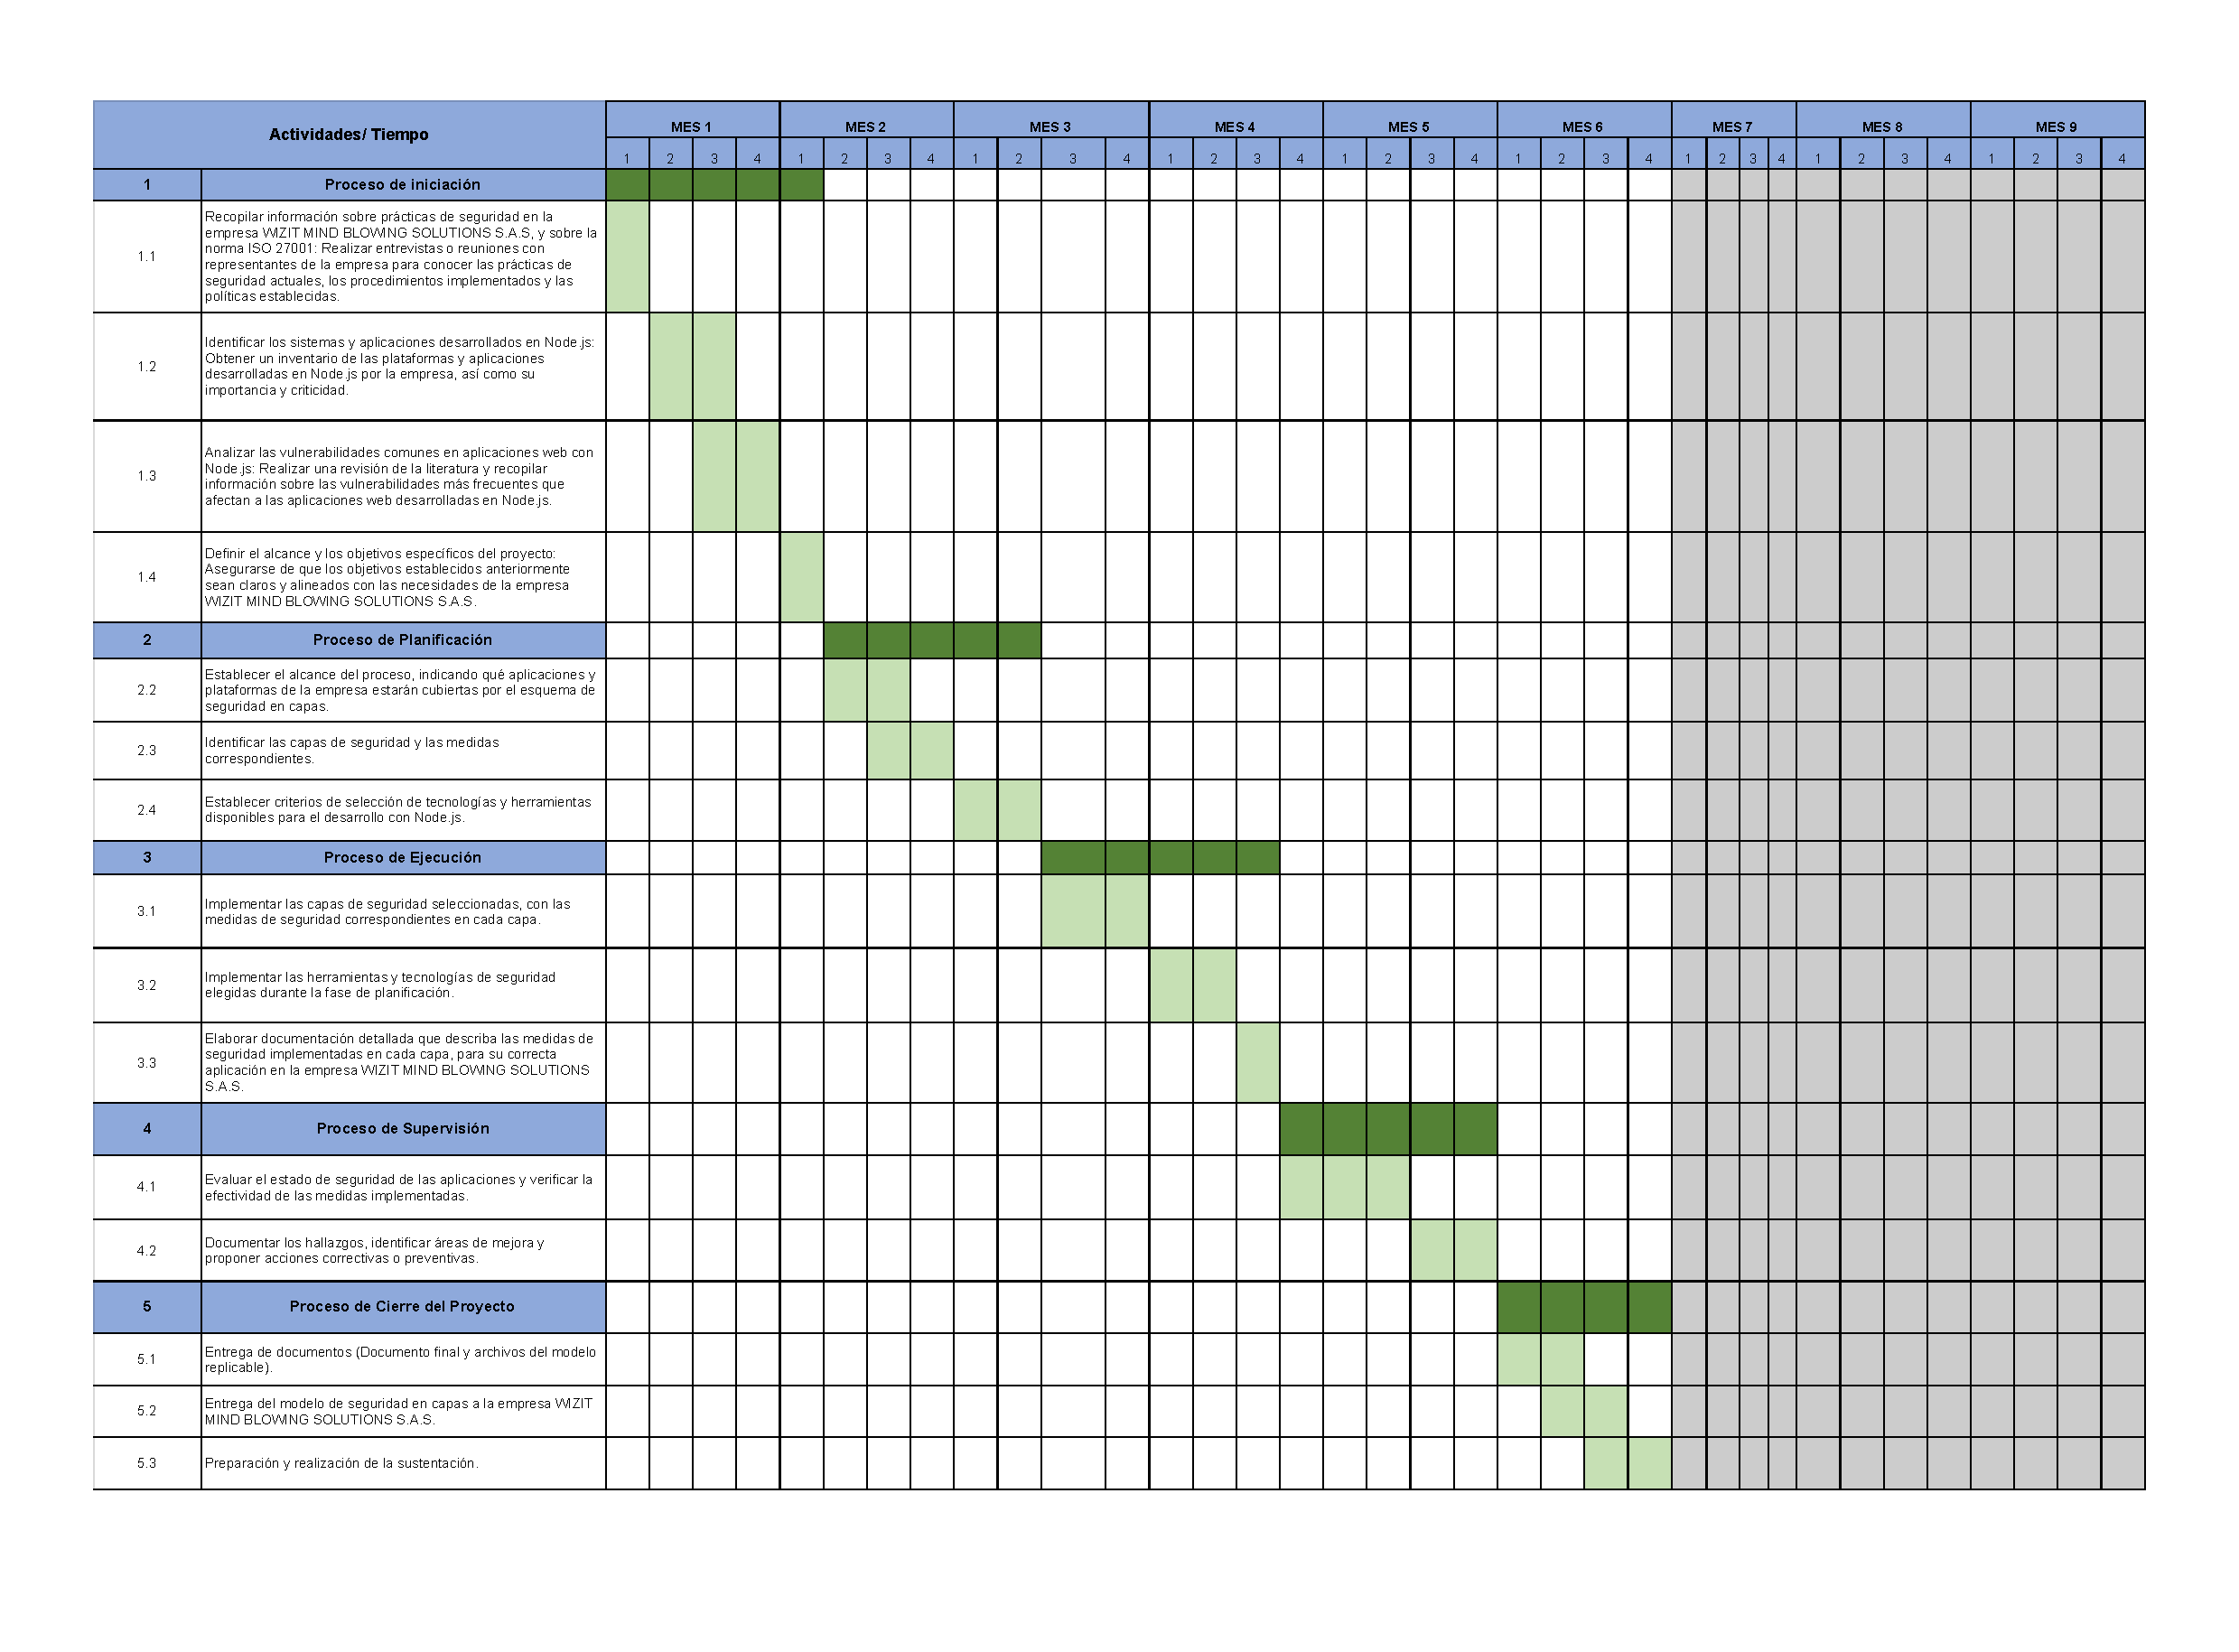
\includepdf[pages=1, scale=0.85, angle=90, offset=1cm 1.5cm, pagecommand={\subsection{CRONOGRAMA}}]{img/Actividades - cronograma.pdf}
\end{landscape}